
% Implications
由于大型河流流域是生态系统服务、经济发展和人类福祉的关键来源,水治理逐渐从主要的地方问题成为国家或国际问题
\cite{best2019,best2020}。
随着远程耦合在联系日益紧密的世界中提出了更多的水治理挑战,水治理的政权转变与不同的人与水的关系相一致\cite{diaz2019}。
这一过程反映了社会如何通过增强其在水社会循环中的适应能力来改变治理实践的建议,IWGI定量地确定了这一转变\cite{loch2020,turton1999}。
科学家和决策者认识到不断变化的治理挑战是至关重要的,因为在一个阶段下开发的模型、制度、工程和方法不一定适用于另一个治理阶段\cite{reyers2018}。

本章研究结果显示在黄河流域在人类主导的近百年间有三种不同的流域治理模式,将它们命名为:集中供水时期(P1: 1965-1978)、治理转型时期(P2: 1979-2001)和适应转向时期(P3: 2002-2013)(图~\ref{ch4:fig:IWGI})。
在水资源压力相对较低的集中供水时期(1965-1978年在黄河流域),水治理因此倾向于通过建造水库和渠道来增加服务(当时主要是供给牲畜和作物用水目的)的供水。
然而,正如当时“人定胜天”的口号所强调的,水资源供应的增加并不符合人与水关系不可逆转的变化;它在不考虑生态保护的情况下急剧增加了用水需求
\cite{zhou2020}。
在同一十年里,灌溉农田和引水设施的迅速扩张使超负荷的黄河流域接近一个临界点,增加供应以满足需求是不切实际的\cite{loch2020}。
自1972年以来,超过$80\%$的地表水被使用,导致河流频繁枯竭,造成了额外的生态问题,如湿地萎缩和生物多样性下降\cite{wang2019c}。
此外,由于水资源压力也限制了工业经济的发展,现有的水治理模式导致了社会-生态危机
\cite{wohlfart2016a}。

治理体制转型的开始(P2: 1979-2001)恰逢“改革开放”后水资源竞争的加剧。
YRB的结果反映了理论分析的结果:在流域总供应稳定的情况下,水资源需求的持续增长可以伴随治理制度的重大变化和整体社会适应能力的快速增强\cite{loch2020}。
作为改变治理机构的先驱,YRB在该政权期间引发了制度变革。这些措施包括,例如,减缓灌溉面积的增长;引领节水基础设施建设;制定中国首个用水配额制度,并初步制定跨境调水方案
\cite{wang2019b,long2020,nickum2021}。
因此,尽管水资源压力仍然存在并增加(由于流量和灵活性的降低),但1999年黄河的最后一次枯竭导致了水治理转型的高潮\cite{wang2019b}。

随后的适应导向制度(P3: 2002-2013)涉及了适应稳定高水资源压力的重大社会转变。
在这种机制中,依赖水资源的地区和部门之间的社会经济权衡发挥了更重要的作用,因此水治理必须实现有效的水资源分配,同时在有限的供水条件下平衡不同的需求
\cite{dalin2015,song2022}。
不同行业和地区对资源的广泛重建,以调整以前制度的刚性配额份额的迫切要求为例,导致对水治理的适应性要求。
许多国家层面的治理实践都是在该制度下提出的,因为缺乏支持高质量发展的政策成为水治理的结构性新挑战
\cite{konar2019}。

总体而言,长江流域的水治理是“改善供给、转变治理、增强适应”的水社会循环总体转型中最突出的例子之一。
随着每个维度的逐渐变化,不同制度的出现在流域尺度上推动了水治理的挑战:这些挑战在转型前主要是经济和环境方面的,但在转型结束后则与社会和政策有关(图~\ref{fig:summary})。
在全球范围内,以水资源短缺和供水困难为代表的资源挑战主要存在于未开发盆地和发展中盆地
\cite{allan2019,speed2013,liu2012a}。
高度控制和发达的盆地(特别是跨界河流)必须主要解决结构性挑战,如水纠纷或缺乏公平,并且可能迫切需要新的灵活、高效的社会政治治理结构
\cite{mirumachi2015}。
IWGI的实施将政权转变与治理挑战联系起来,从而提供了一种全面而直接的方式来解释水治理与水社会转型之间的相互关系。

\begin{figure*}[htbp!]
	\centering
	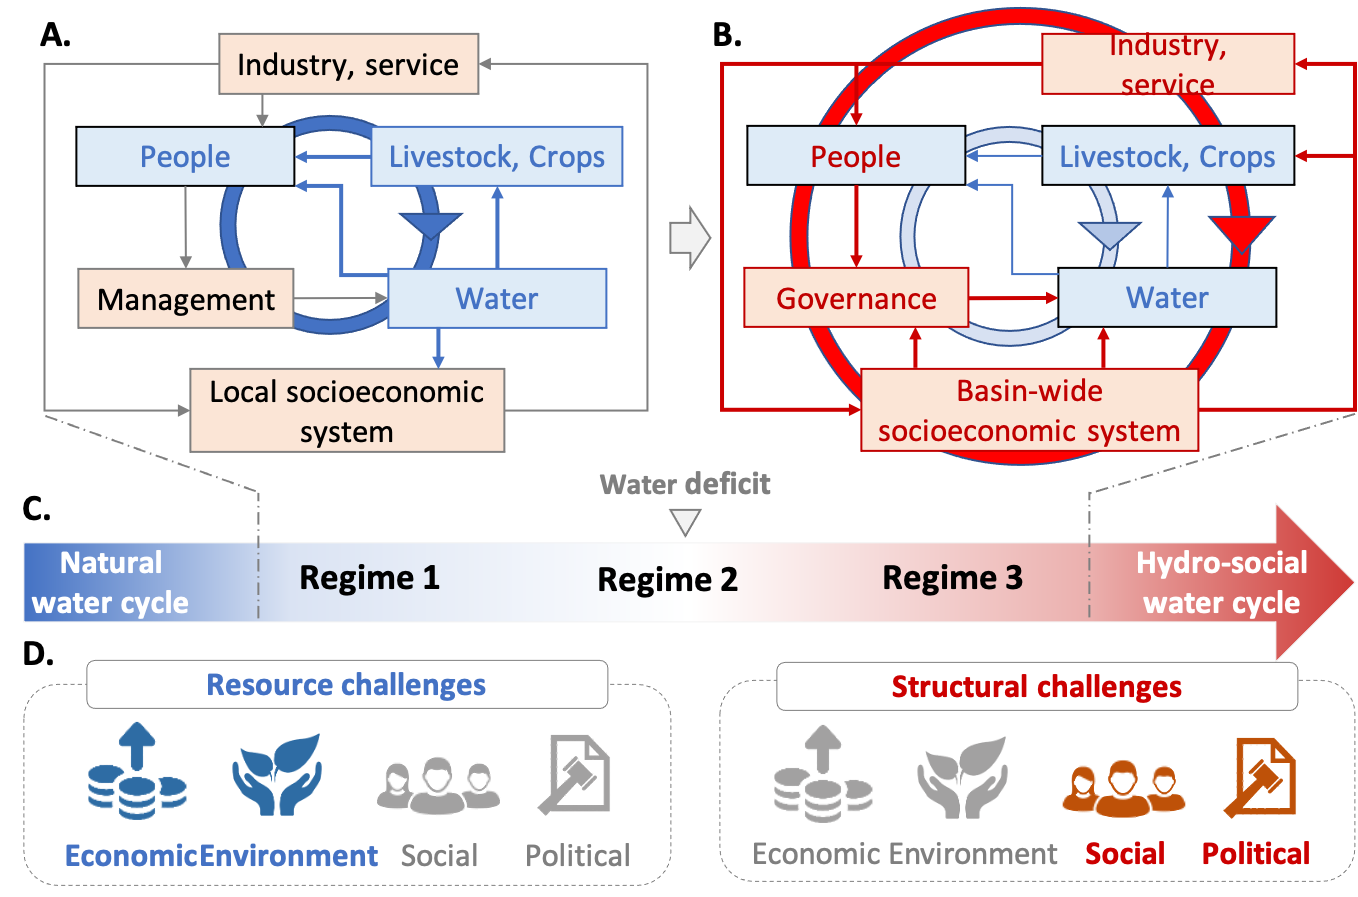
\includegraphics[width=\textwidth]{img/ch4/transition.png}
	\caption{
		水社会循环与水治理机制的转型模式。蓝色代表自然水循环,红色代表社会经济反馈。
        \textbf{A.}随着社会经济系统的发展,非供应用水需求增加;同时,通过工程提高的适应能力使人们能够管理水资源以缓解水资源压力。
        \textbf{B.}随着进一步的人为干预,供应用水和非供应用水之间的权衡变得突出;整个流域的社会经济系统需要更有组织的水治理。
        因此,\textbf{C. the hydrosocial water cycle transition}与水治理体制的转变相关。治理体制转型发生在水资源亏缺之后,适应能力快速增长。
        通过过渡制度,水治理主要面临经济和环境挑战,但随后面临社会和政策挑战。
	}
	\label{fig:summary}
\end{figure*}


%* limitations & direction
该方法的主要局限性之一是缺乏全球范围内的长期数据,这意味着在全面识别和更广泛地应用IWGI之间仍然存在差距。
然而,我们建议,所有的水治理问题都会导致“谁获得水、何时获得水以及如何获得水”的改变,因此监测水压力、水服务的目的和水分配模式确实有帮助。
不同方面的指标选择可根据现有数据集进行调整;底层组件之间的联系对于全面理解治理机制中的过渡仍然至关重要。
在当今世界,水动力学从生物物理控制体制向水社会控制体制的转变似乎越来越普遍;应对治理挑战的综合战略必须成为复杂的人-水系统的核心
\cite{cumming2018,cumming2014,jaeger2019}。
尽管河流流域在水管理技术和用水效率方面已经有所改善,但许多流域仍在接近人类-水系统可能崩溃的地方、区域和地球边界
\cite{gleeson2020, wang-erlandsson2022}。
更深入地理解治理,结合非线性政权转移和转型的思想,应该有助于将治理的重点转向维持盆地社会-生态系统的恢复力和提高其可持续性
\cite{falkenmark2019}。
